\subsection{KNN}
En esta sección definimos:
\begin{itemize}
	\item $k$: cantidad de vecinos a considerar en el algoritmo $kNN$.
\end{itemize}
El análisis sobre el algoritmo $KNN$ ($k$ vecinos más cercanos) se realiza para distintos valores de $k$. La idea detrás de esta elección de la variable busca entender la variación en la efectividad (cantidad de aciertos) del algoritmo.
\\
Para ello variamos $k$ desde $1$ hasta $30$ para ver cual era el comportamiento que se obtenía.
\\
Para cada uno de los $k$s realizamos dos corridas con diferentes k-folds.
\\
El procedimiento de este algoritmo comienza, por cada imágen que queremos averiguar a que dígito pertenece, con su vectorización. Luego resta el resultado a cada uno de los vectores imágen y calcula la norma 2 para saber en cuanto difieren con cada una de las imágenes.
Todos esos resultados se acumulan en una cola de prioridad que los ordena de menor a mayor, según las diferencias entre la imágen la cual se quiere averiguar a que clase pertenece y todas las imágenes de la base de datos etiquetada.
\\
Como siguiente paso se toman los $k$ primeros elementos de la cola de prioridad y se verifica a que dígito se corresponden para luego saber cual es el dígito que recibió mas "votos" y ver si se produjo un acierto o no.
Por lo tanto, una supocición preliminar es que a mayor cantidad de vecinos (o sea, $k$) menor va a ser la cantidad de aciertos, ya que se empiezan a mirar los elementos de menor prioridad de la cola, eso significa, que se cuentan primero las imágenes que más difieren y eso puede hacer que las chances de acertar el dígito correcto disminuyan.

\subsubsection{Cantidad de vecinos}
Como ya digimos, para analizar cual es el mejor número de vecinos para el cual el algoritmo $KNN$  da una mayor cantidad de aciertos, optamos por variar la cantidad de $k$ vecinos a tomar.

Se prueba entonces el algoritmo $KNN$ para los siguientes valores: $1,2,3,4,...,30$.
\\
Para el primer k-fold con el que probamos, que contaba con 4200 imagenes para testear, obtuvimos el siguiente grafico:
\\
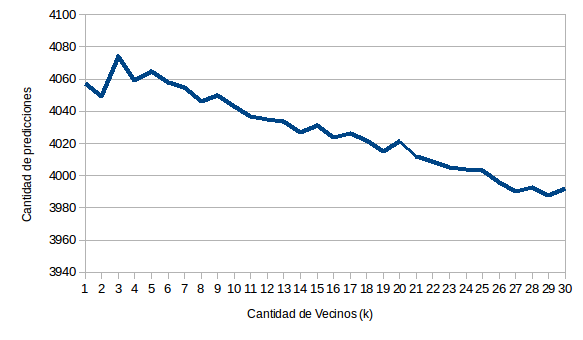
\includegraphics[scale=0.55]{nuevosResultados/knn/1.png}\\

Los resultados son bastante sorprendentes. Para valores muy pequeños de k (k=1,K=2) podemos observar que los resultados son peores que para $k=3$ lo cual no esperabamos que sucediera. Luego para valores mas grandes si se observa lo que nos decía la intuición, tal que para un gran numero de vecinos se empiezan a perder aquellos que son realmente relevantes.
\\
Aun así estos resultados no nos dejaron satisfechos así que realizamos otro k-fold diferente, con otras 4200 imagenes distintas para testear para ver si obteníamos resultados similares o el k-fold anteriór padecía de alguna particularidad extraordinaria.
\\
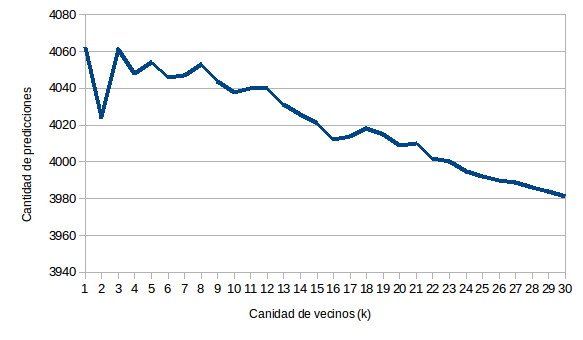
\includegraphics[scale=0.55]{nuevosResultados/knn/2.png}\\
\\
Los resultados que obtenemos son muy similares a los anteriores, por lo que concluímos que $k=3$ es el valor optimo de vecinos a tomar.
\\
Ademas para estas dos tests realizamos una medición de tiempos para ver como se comportaba el algoritmo frente a un cambio en la cantidad de vecinos. Los resultados pueden verse en el siguente grafico:

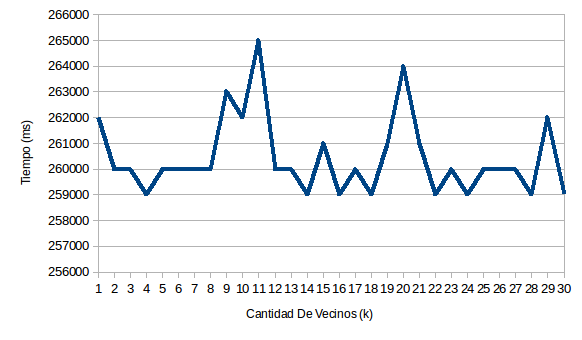
\includegraphics[scale=0.55]{nuevosResultados/knn/1temp.png}\\

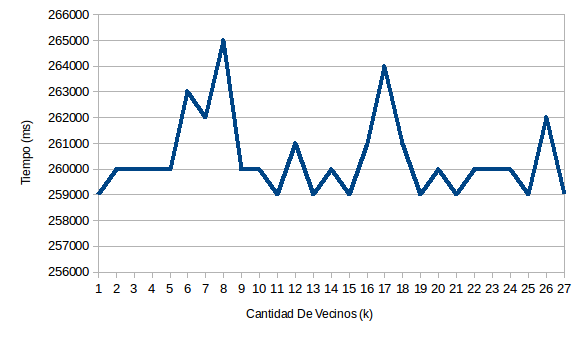
\includegraphics[scale=0.55]{nuevosResultados/knn/2temp.png}\\

Como puede observarse, los tiempos de los algoritmos no se ven muy afectados por la variación en la cantidad de vecinos. Es muy probable que esto se deba a que el algoritmo debe comparar a la imagen que se desea comparar contra un numero muy extenso de imagenes, estan en el mismo orden de magnitud, bla bla...
\completar

Usamos $k=3$ porque es el mejor.

\subsection{PCA}
\subsubsection{Cantidad de vecinos y $\alpha$ inicial}
En esta sección definimos:
\begin{itemize}
	\item $\alpha$: a la cantidad de componentes principales a tomar para el $PCA$.
	\item $k$: cantidad de vecinos a considerar en el algoritmo $kNN$.
\end{itemize}
En primera instancia vamos a utlilizar k-folds para intentar determinar el mejor $\alpha$ posible. Supondremos en este momento que el mejor $k$ para este caso es tambien $3$ (aunque esto podría no ser asi) y luego testearemos si esto es asi o si para el $\alpha$ encontrado existe algun otro $k$ optimo.
\\
Enfocamos nuestro análisis en obtener un valor óptimo de $\alpha$. Para este fin, realizamos varias corridas tratando de maximizar la performance del algoritmo. Dado que este parámetro representa la cantidad de componentes principales a tener en cuenta y teniendo en mente el funcionamiento del algoritmo de PCA, es esperable que valores pequeños no sean beneficiosos (teniendo en cuenta que el máximo a considerar es bastante elevado), pero dado que PCA las ordena en base a su relevancia, se alcance un valor óptimo sin necesidad de considerarlas todas. Para un mismo k-fold con 4200 imagenes para testear, tomamos $\alpha$ desde $1$ hasta $50$ y graficamos lo obtenido:

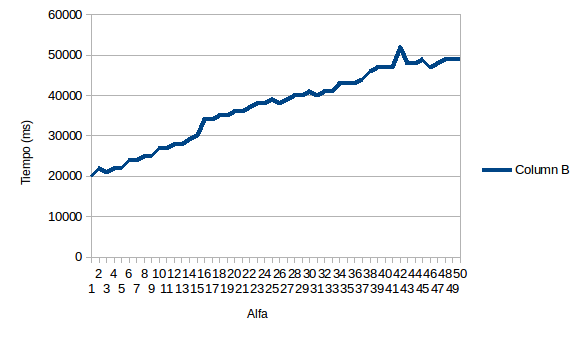
\includegraphics[scale=0.75]{nuevosResultados/pca/pca1.png}\\

Puede verse que para valores pequeños, aumentar en uno el $\alpha$ produce un gran aumento de aciertos. Por ejemplo, para $\alpha$ igual a $1$ se obtienen 1107 aciertos, mientras que para $\alpha$ igual a $2$ se obtienen 1693 aciertos, esto es un $52\%$ mas de aciertos.
\\
Para valores mas grandes de $\alpha$ (al rededor de $\alpha = 12$) esta tendencia empieza estabilizarse. Por ejemplo para $\alpha = 12$ se obtienen $3865$ imagenes correctamente predecidas, pero para $\alpha = 13$ se obtienen 3881 imagenes correctas, esto es el crecimiento de aciertos es de menos de un $1\%$.
\\
Ademas, para este k-fold realizamos una medición de tiempos, que se puede ver a continuación:

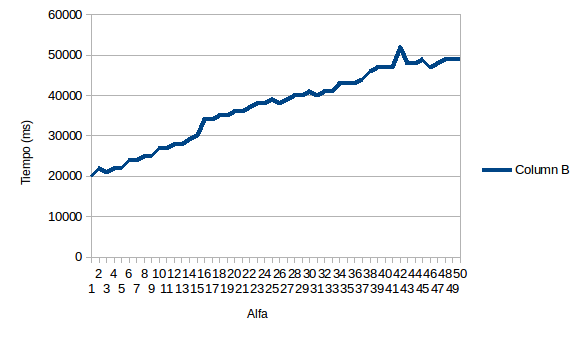
\includegraphics[scale=0.75]{nuevosResultados/pca/pca1.png}\\

En este grafico se puede ver que aumentar el $\alpha$ produce un aumento lineal de los tiempos de ejecución, de lo que se desprende que aumentar la cantidad valores principales no resulta gratuito y tiene cierto costo asociado.
\\
Ademas aumentar de manera desmedida el $\alpha$ puede probocar lo que en machine learning se denomina 'Overfiting'.
\inventarReferencia
\\
Debido a todas las razones expuestas consideramos que con $\alpha$ igual a $14$ será el mejor valor que podemos tomar.
\\

%falta retestear esto de abajo

La segunda prueba a realizar es, fijando un valor de $\alpha$, analizar para que cantidad de vecinos se obtiene la mayor cantidad de aciertos.
Después de aplicar el algoritmo $PCA$, se aplica el algoritmo $KNN$, armando una cola de prioridad para los resultados de aplicar el algoritmo $KNN$. Lo que se hace es tomar dos imágenes, restarlas y aplicarle la norma 2 para saber en cuanto difiere una imagen de la otra. En la cola de prioridad se encuentran por delante los valores más chicos, o sea, las imágenes del test que más cerca de coincidir están con respecto a la imágen de la base de datos.
Por lo tanto, si elegimos una mayor cantidad de vecinos, pueden pasar dos cosas:

\begin{itemize}
  \item Que sea beneficioso ya que a mayor cantidad de pruebas vamos a tener mas aciertos
  \item Que sea malicioso ya que a mayor cantidad de pruebas vamos a obtener peores datos, o sea, vamos a mirar las imágenes que menos coiciden con la imagen de prueba de la base de datos.
\end{itemize}

